\documentclass[11pt]{article}

%% for bibliography
\usepackage[natbibapa]{apacite}
\bibliographystyle{apacite} 

% size of plots and tables
\usepackage{adjustbox} 

% section numbering
\usepackage{chngcntr}
\counterwithin{table}{section}
\counterwithin{figure}{section}

% header of paper
\title{This is my work in R}
\author{
        MyFirstName MyLastName\\
        ThisIs mySchoolProgramName\\
        ThisIs UniversityName\\
        City, ZipCope, \underline{Country}\\
        \texttt{username@the.rest}
}
%\date{August 23, 2022} %manually
\date{\today}  %automatic


% every "begin: needs and "end"
\usepackage{Sweave}
\begin{document}

\Sconcordance{concordance:WorkInR_forPrinter.tex:WorkInR_forPrinter.Rnw:%
1 28 1 1 0 11 1 1 8 18 1 1 5 11 1 1 16 18 0 1 2 10 1 1 11 4 1 2 2 12 1 %
1 8 14 0 1 2 5 1 1 8 4 1 2 2 13 1 1 8 3 1 1 6 31 0 1 2 4 1 1 6 31 0 1 2 %
11 1 1 11 1 13 4 1 2 2 22 1 1 14 3 1 2 2 24 1}

\maketitle 

\begin{abstract}
This is an example of an abstract in a paper. This is an example of an abstract in a paper. This is an example of an abstract in a paper. This is an example of an abstract in a paper.This is an example of an abstract in a paper.This is an example of an abstract in a paper.This is an example of an abstract in a paper.

\end{abstract}

% a chunk hidden (echo=FALSE) with some setup
% chunk has its own name 


\section*{Introduction} % * to unnumber

This is just my intro to my nice paper. This is just my intro to my nice paper.This is just my intro to my nice paper. This is just my intro to my nice paper.This is just my intro to my nice paper. This is just my intro to my nice paper.This is just my intro to my nice paper. This is just my intro to my nice paper.This is just my intro to my nice paper. This is just my intro to my nice paper.This is just my intro to my nice paper. This is just my intro to my nice paper.

This is just my intro to my nice paper. This is just my intro to my nice paper.This is just my intro to my nice paper. This is just my intro to my nice paper.This is just my intro to my nice paper. This is just my intro to my nice paper.This is just my intro to my nice paper. This is just my intro to my nice paper.


\section{Exploring Tables}\label{explo-tables} % label for crossref

%footnote coming
Another section. I will use a footnot now \footnote{This is a footnote.}. I will soon use cross-ref.I will soon use cross-ref.I will soon use cross-ref.I will soon use cross-ref. I will soon use cross-ref. I will soon use cross-ref.I will soon use cross-ref.I will soon use cross-ref.I will soon use cross-ref.I will soon use cross-ref. I will soon use cross-ref. I will soon use cross-ref.
%cross-ref coming

%cross-ref coming
I will soon use cross-ref.I will soon use cross-ref: as we see in Section \ref{catexplor}.



\subsection{Exploring Categorical Data}\label{catexplor}

Here, I continue doing this nice work, I hope you like it and read it. It has been a very hard work.Here, I continue doing this nice work, I hope you like it and read it. It has been a very hard work.Here, I continue doing this nice work, I hope you like it and read it. It has been a very hard work.Here, I continue doing this nice work, I hope you like it and read it. It has been a very hard work.Here, I continue doing this nice work, I hope you like it and read it. It has been a very hard work.Here, I continue doing this nice work, I hope you like it and read it. It has been a very hard work.

I hope you like it and read it. It has been a very hard work.Here, I continue doing this nice work, I hope you like it and read it. It has been a very hard work.Here, I continue doing this nice work, I hope you like it and read it. It has been a very hard work.Here, I continue doing this nice work, I hope you like it and read it. It has been a very hard work.Here, I continue doing this nice work, I hope you like it and read it. It has been a very hard work.

You can see the statistics of a categorical variable in Table \ref{catexploreTable}.

%the chunk name is NOT used in cross-ref for table.
%Table is created and displayed.

\begin{table}

\caption{This is a table\label{catexploreTable}}
\centering
\begin{tabular}[t]{l|r|r|r}
\hline
Democracy Index & count & pct & pct\_cumm\\
\hline
veryLow & 53 & 33.76 & 33.76\\
\hline
low & 31 & 19.75 & 53.50\\
\hline
medium & 53 & 33.76 & 87.26\\
\hline
good & 0 & 0.00 & 87.26\\
\hline
veryGood & 20 & 12.74 & 100.00\\
\hline
\end{tabular}
\end{table}

%%%%%%

You can see this variable plotted in Figure \ref{catBarplot} on page \pageref{catBarplot}.

% NO need for figure caption in chunk header.
% Object will be created BUT NOT plotted
% the chunk name IS NOT used in cross-ref for figure


% Latex will use this code for plotting
\begin{figure}[h]
\centering
\begin{adjustbox}{width=7cm,height=5cm} %resize
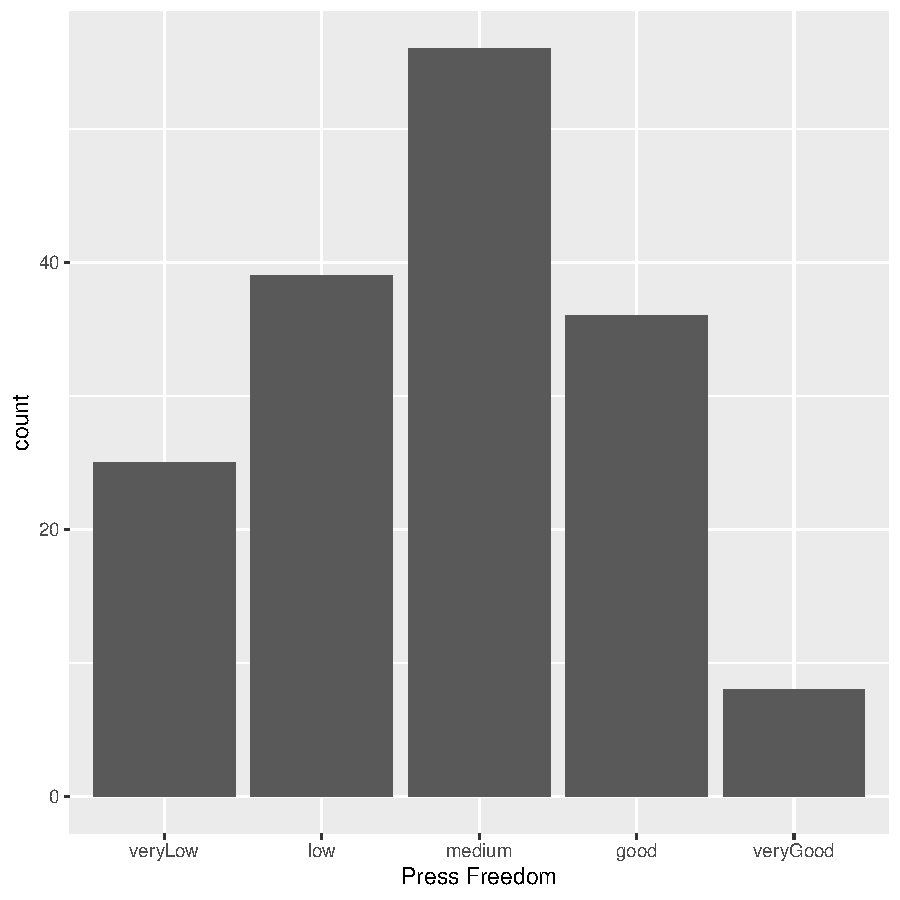
\includegraphics{WorkInR_forPrinter-catBarplot}
\end{adjustbox}
\caption{Press Freedom Index in the World}  %title
\label{catBarplot} % for cross-ref
\end{figure}



\subsection{Exploring Numerical Data}\label{numexplo}

Here, I continue doing this nice work, I hope you like it and read it. It has been a very hard work.Here, I continue doing this nice work, I hope you like it and read it. It has been a very hard work.Here, I continue doing this nice work, I hope you like it and read it. It has been a very hard work.Here, I continue doing this nice work, I hope you like it and read it. It has been a very hard work.Here, I continue doing this nice work, I hope you like it and read it. It has been a very hard work.Here, I continue doing this nice work, I hope you like it and read it. It has been a very hard work.Here, I continue doing this nice work, I hope you like it and read it. It has been a very hard work.Here, I continue doing this nice work, I hope you like it and read it. It has been a very hard work.Here, I continue doing this nice work, I hope you like it and read it. It has been a very hard work.

Here, I continue doing this nice work, I hope you like it and read it. It has been a very hard work.Here, I continue doing this nice work, I hope you like it and read it. It has been a very hard work.

% Table created by stargazer v.5.2.3 by Marek Hlavac, Social Policy Institute. E-mail: marek.hlavac at gmail.com
% Date and time: Mon, Aug 22, 2022 - 15:42:24
\begin{table}[!htbp] \centering 
  \caption{Stat summary for nummeric vars} 
  \label{summaryNumeric} 
\footnotesize 
\begin{tabular}{@{\extracolsep{5pt}}lccccccc} 
\\[-1.8ex]\hline 
\hline \\[-1.8ex] 
Statistic & \multicolumn{1}{c}{N} & \multicolumn{1}{c}{Mean} & \multicolumn{1}{c}{St. Dev.} & \multicolumn{1}{c}{Min} & \multicolumn{1}{c}{Pctl(25)} & \multicolumn{1}{c}{Pctl(75)} & \multicolumn{1}{c}{Max} \\ 
\hline \\[-1.8ex] 
DemocracyIndex & 157 & 2.38 & 1.30 & 1 & 1 & 3 & 5 \\ 
mili\_pctGDP & 166 & 2.07 & 1.55 & 0.20 & 1.10 & 2.48 & 10.00 \\ 
\hline \\[-1.8ex] 
\end{tabular} 
\end{table} 
% Use of R object inline
In the Table \ref{summaryNumeric}, you realize that the mean of military expenditure is {\bf2.07228915662651}.

It would be good to see a boxplot, check Figure \ref{numBoxplot} below.


\begin{figure}[h]
\centering
\begin{adjustbox}{width=7cm,height=5.5cm,clip,trim=0cm 0.5cm 0cm 0cm} 
\includegraphics{WorkInR_forPrinter-numBoxplot}
\end{adjustbox}
\caption{Money spent per country on Military stuff}  
\label{numBoxplot} 
\end{figure}

%%%%% A citation: author(year)
Boxplots were introduced by \citet{tukey_exploratory_1977}.


%%%%
\section{My Regression}\label{regre}

Several times we need regression.



This is a nice summary for two regressions:

% Table created by stargazer v.5.2.3 by Marek Hlavac, Social Policy Institute. E-mail: marek.hlavac at gmail.com
% Date and time: Mon, Aug 22, 2022 - 15:42:24
\begin{table}[!htbp] \centering 
  \caption{Regression Models} 
  \label{regs1} 
\begin{tabular}{@{\extracolsep{5pt}}lcc} 
\\[-1.8ex]\hline 
\hline \\[-1.8ex] 
 & \multicolumn{2}{c}{\textit{Dependent variable:}} \\ 
\cline{2-3} 
\\[-1.8ex] & \multicolumn{2}{c}{mili\_pctGDP} \\ 
\\[-1.8ex] & (1) & (2)\\ 
\hline \\[-1.8ex] 
 DemocracyIndex & $-$0.423$^{***}$ & $-$0.535$^{***}$ \\ 
  & (0.090) & (0.128) \\ 
  & & \\ 
 IndexofEconomicFreedom &  & 0.230 \\ 
  &  & (0.149) \\ 
  & & \\ 
 Constant & 3.083$^{***}$ & 2.730$^{***}$ \\ 
  & (0.245) & (0.291) \\ 
  & & \\ 
\hline \\[-1.8ex] 
Observations & 157 & 154 \\ 
R$^{2}$ & 0.124 & 0.126 \\ 
Adjusted R$^{2}$ & 0.119 & 0.114 \\ 
Residual Std. Error & 1.464 (df = 155) & 1.434 (df = 151) \\ 
F Statistic & 22.008$^{***}$ (df = 1; 155) & 10.857$^{***}$ (df = 2; 151) \\ 
\hline 
\hline \\[-1.8ex] 
\textit{Note:}  & \multicolumn{2}{r}{$^{*}$p$<$0.1; $^{**}$p$<$0.05; $^{***}$p$<$0.01} \\ 
\end{tabular} 
\end{table} 

You can also do this: You can also do this:You can also do this:You can also do this: You can also do this:You can also do this:You can also do this: You can also do this:You can also do this:You can also do this: You can also do this:You can also do this:You can also do this: You can also do this:You can also do this:You can also do this: You can also do this:You can also do this:You can also do this: You can also do this:You can also do this:You can also do this: You can also do this:You can also do this:
\pagebreak

% Table created by stargazer v.5.2.3 by Marek Hlavac, Social Policy Institute. E-mail: marek.hlavac at gmail.com
% Date and time: Mon, Aug 22, 2022 - 15:42:24
\begin{table}[!htbp] \centering 
  \caption{Regression Models} 
  \label{regs2} 
\begin{tabular}{@{\extracolsep{5pt}}lcc} 
\\[-1.8ex]\hline 
\hline \\[-1.8ex] 
 & \multicolumn{2}{c}{\textit{Dependent variable:}} \\ 
\cline{2-3} 
\\[-1.8ex] & \multicolumn{2}{c}{Military Expenditure (percent of GDP)} \\ 
\\[-1.8ex] & (1) & (2)\\ 
\hline \\[-1.8ex] 
 Democracy & $-$0.423$^{***}$ & $-$0.535$^{***}$ \\ 
  & (0.090) & (0.128) \\ 
  & & \\ 
 Economic Freedom &  & 0.230 \\ 
  &  & (0.149) \\ 
  & & \\ 
 Constant & 3.083$^{***}$ & 2.730$^{***}$ \\ 
  & (0.245) & (0.291) \\ 
  & & \\ 
\hline \\[-1.8ex] 
Observations & 157 & 154 \\ 
R$^{2}$ & 0.124 & 0.126 \\ 
Adjusted R$^{2}$ & 0.119 & 0.114 \\ 
Residual Std. Error & 1.464 (df = 155) & 1.434 (df = 151) \\ 
F Statistic & 22.008$^{***}$ (df = 1; 155) & 10.857$^{***}$ (df = 2; 151) \\ 
\hline 
\hline \\[-1.8ex] 
\textit{Note:}  & \multicolumn{2}{r}{$^{*}$p$<$0.1; $^{**}$p$<$0.05; $^{***}$p$<$0.01} \\ 
\end{tabular} 
\end{table} 
I hope you like what you see in the Table \ref{regs1} and in Table \ref{regs2}. You can learn more on regression in 
other book \citep[150-160]{petrie_introduction_2016}

%%%%


\section{Other plots}\label{otherPlots}

\subsection{A word cloud}\label{wordPlot}

Let me show a nice word cloud.Let me show a nice word cloud.Let me show a nice word cloud.Let me show a nice word cloud.Let me show a nice word cloud.Let me show a nice word cloud.Let me show a nice word cloud.Let me show a nice word cloud.Let me show a nice word cloud.Let me show a nice word cloud.Let me show a nice word cloud.Let me show a nice word cloud. Let me show a nice word cloud.Let me show a nice word cloud.Let me show a nice word cloud.Let me show a nice word cloud.Let me show a nice word cloud.Let me show a nice word cloud.




\begin{figure}[h]
\centering
\begin{adjustbox}{width=10cm,height=10cm,clip,trim=0cm 2cm 0cm 2cm} 
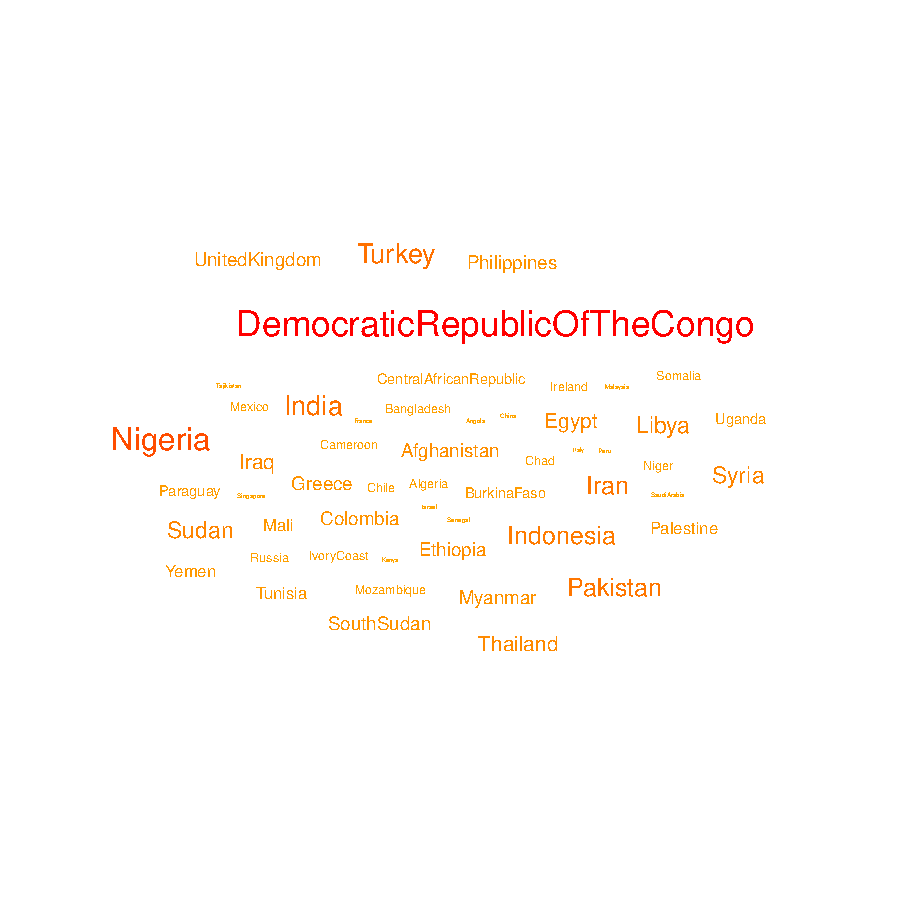
\includegraphics{WorkInR_forPrinter-theCloudPlot}
\end{adjustbox}
\caption{Nations by presence of rebel movements.}  
\label{theCloudPlot} 
\end{figure}


Above you see our Figure \ref{theCloudPlot}. Here, I continue doing this nice work, I hope you like it and read it. It has been a very hard work.Here, I continue doing this nice work, I hope you like it and read it. It has been a very hard work.Here, I continue doing this nice work, I hope you like it and read it. It has been a very hard work.Here, I continue doing this nice work, I hope you like it and read it. It has been a very hard work.Here, I continue doing this nice work, I hope you like it and read it. It has been a very hard work.Here, I continue doing this nice work, I hope you like it and read it. It has been a very hard work.Here, I continue doing this nice work, I hope you like it and read it. It has been a very hard work.Here, I continue doing this nice work, I hope you like it and read it. It has been a very hard work.Here, I continue doing this nice work, I hope you like it and read it. It has been a very hard work.

It has been a very hard work.Here, I continue doing this nice work, I hope you like it and read it.

It has been a very hard work.Here, I continue doing this nice work, I hope you like it and read it. It has been a very hard work.Here, I continue doing this nice work, I hope you like it and read it. 

You can read something interesting somewhere else \citep{lipman_art_2022}.

\subsection{A map}\label{mapPlot}

Let me show a nice map.Let me show a nice map.Let me show a nice map.Let me show a nice map.Let me show a nice map.Let me show a nice map.Let me show a nice map.Let me show a nice map.Let me show a nice map.Let me show a nice map.Let me show a nice map.Let me show a nice map.

Let me show a nice map.Let me show a nice map.Let me show a nice map.Let me show a nice map.Let me show a nice map.Let me show a nice map.Let me show a nice map.Let me show a nice map.Let me show a nice map.Let me show a nice map.Let me show a nice map.Let me show a nice map.

Let me show a nice map.Let me show a nice map.Let me show a nice map.Let me show a nice map.Let me show a nice map.Let me show a nice map.Let me show a nice map.Let me show a nice map.Let me show a nice map.Let me show a nice map.Let me show a nice map.Let me show a nice map in Figure \ref{theMapPlot}.



\begin{figure}[h]
\centering
\begin{adjustbox}{width=10cm,height=10cm} 
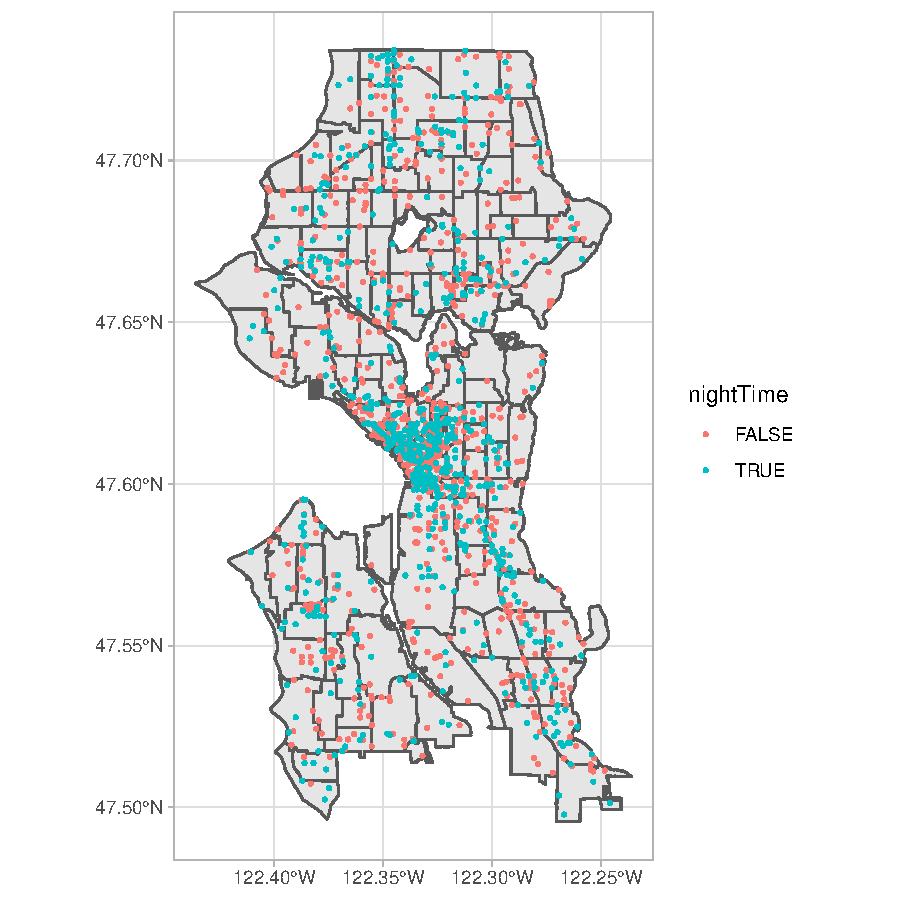
\includegraphics{WorkInR_forPrinter-theMapPlot}
\end{adjustbox}
\caption{Calls to 911 by time of day.}  
\label{theMapPlot} 
\end{figure}


Here, I continue doing this nice work, I hope you like it and read it. It has been a very hard work.Here, I continue doing this nice work, I hope you like it and read it. It has been a very hard work.Here, I continue doing this nice work, I hope you like it and read it. It has been a very hard work.Here, I continue doing this nice work, I hope you like it and read it. 

Review other authors 
(\citealp[120-160]{brunsdon_introduction_2015};
\citealp[also, see][]{camara_spatial_nodate}) to know more.







\newpage
%%%%% adding bibliography


%\bibliographystyle{apacite}
%\renewcommand{\refname}{Bibliography}
\bibliography{FGVexample}

\end{document}
